  \chapter{Design og implementering}


\section{Software Design}

\subsection{Devkit8000}

\subsubsection{Candydriver}
Candydriveren sørger for SPI-kommunikationen fra Devkit8000 til PSoC0. SPI-kommunikationen er implementeret med SPI bus nummer 1, SPI chip-select 0 og en hastighed på 1 MHz (et godt stykke under max på 20 MHz for en sikkerhedsskyld). Desuden starter clocken højt og data ændres på falling edge og aflæses på rising edge. Dermed bliver SPI Clock Mode 3. Derudover sendes der 8 bit pr transmission, hvilket passer med SPI-protokollen for projektet.\\
For at kunne anvende driveren, når SPI er tilsluttet, er der oprettet et hotplugmodul, som fortæller kernen, at der er et SPI device, som matcher driveren. Det kan SPI-forbindelsen ikke selv gøre, som usb fx kan. Selve driveren er i candygun.c opbygget som en char driver. For at holde forskellige funktionaliteter adskilt er alle funktioner, der har med SPI at gøre, implementeret i filen candygun-spi-c. Så når der fx skal requestes en SPI ressource i init-funktionen i candygun.c, så anvender driveren en funktion fra candygun-spi.c til det. I probe-funktionen sættes bits\textunderscore per\textunderscore word til 8, da vi sender otte bit som nævnt tidligere. I exit-funktionen anvender candygun.c igen en funktion fra candygun-spi.c - denne gang til at frigive SPI ressourcen. I write-metoden gives der data med fra brugeren. I dette tilfælde udgøres brugeren af Interface driveren og dataet er en 8 bit kommando fra SPI-protokollen. Dog er dataet fra brugeren i første omgang læst ind som en charstreng. I write-metoden bliver det så lavet om til en int.  For at overføre dataet på en sikker måde anvendes funktionen copy\textunderscore from\textunderscore user() til at overføre data fra brugeren. Write-funktionen fra candygun.c anvender derefter en write-funktion fra candygun-spi.c, hvor den sender brugerinputtet med. I den spi-relaterede write-funktion bliver bruger inputtet lagt i transfer bufferen og der NULL bliver lagt i receive bufferen, og med spi\textunderscore sync-funktionen bliver det sendt. \\ 
Ofte ville der en spi read-funktion først indeholde en write-del, som fortalte SPI-slaven, hvad der skulle læses over i bufferen. Det ville typisk efterfølges af et delay og så en read-del. Men i dette projekt skal der ofte afventes et brugerinput, som ikke kan styres af et fast delay, og der skal generelt sendes en aktiv kommando før der læses. Derfor er det besluttet at read-funktionen kun indeholder en read-del i transmissionen. Dermed skal write-funktionen altid aktivt anvendes inden der læses, da PSoC0 ellers ikke ved, hvad der skal gøres/lægges i bufferen.\\
Når funktionen har modtaget resultatet fra transmissionen returneres det til brugeren med funktionen copy\textunderscore to\textunderscore user(), som igen sørger for at overførslen af data foregår på en sikker måde.



\subsubsection{Interfacedriver}
Interface driveren er bindeled mellem brugergrænsefladen og candydriveren. Interface driveren er implementeret i c++ og opbygget med klasserelationen arv. Den indeholder tre funktioner til use case 2. De håndterer test af de forskellige kommunikationsforbindelser i systemet. Der er en basisklasse, ICandyGun, som er abstrakt, da alle metoder er virtuelle. Derudover er der to afledte klasser, SimulCandyGun og RealCandyGun. SimulCandyGun simulerer svaret på funktionerne ved brug af rand()-funktionen. Den sikrer at brugergrænsefladen kan testes uden at være forbundet til det resterende system. RealCandyGun klassen implementerer de rigtig funktioner med forbindelse til det restende system, og anvender de nødvendige funktioner til at skrive til og læse fra et kernemodul. På figur \ref{fig:IDriverKlasseDiagram} ses klassediagrammet for arvehierarkiet i Interface Driveren. 

\begin{figure}[H]
	\centering
	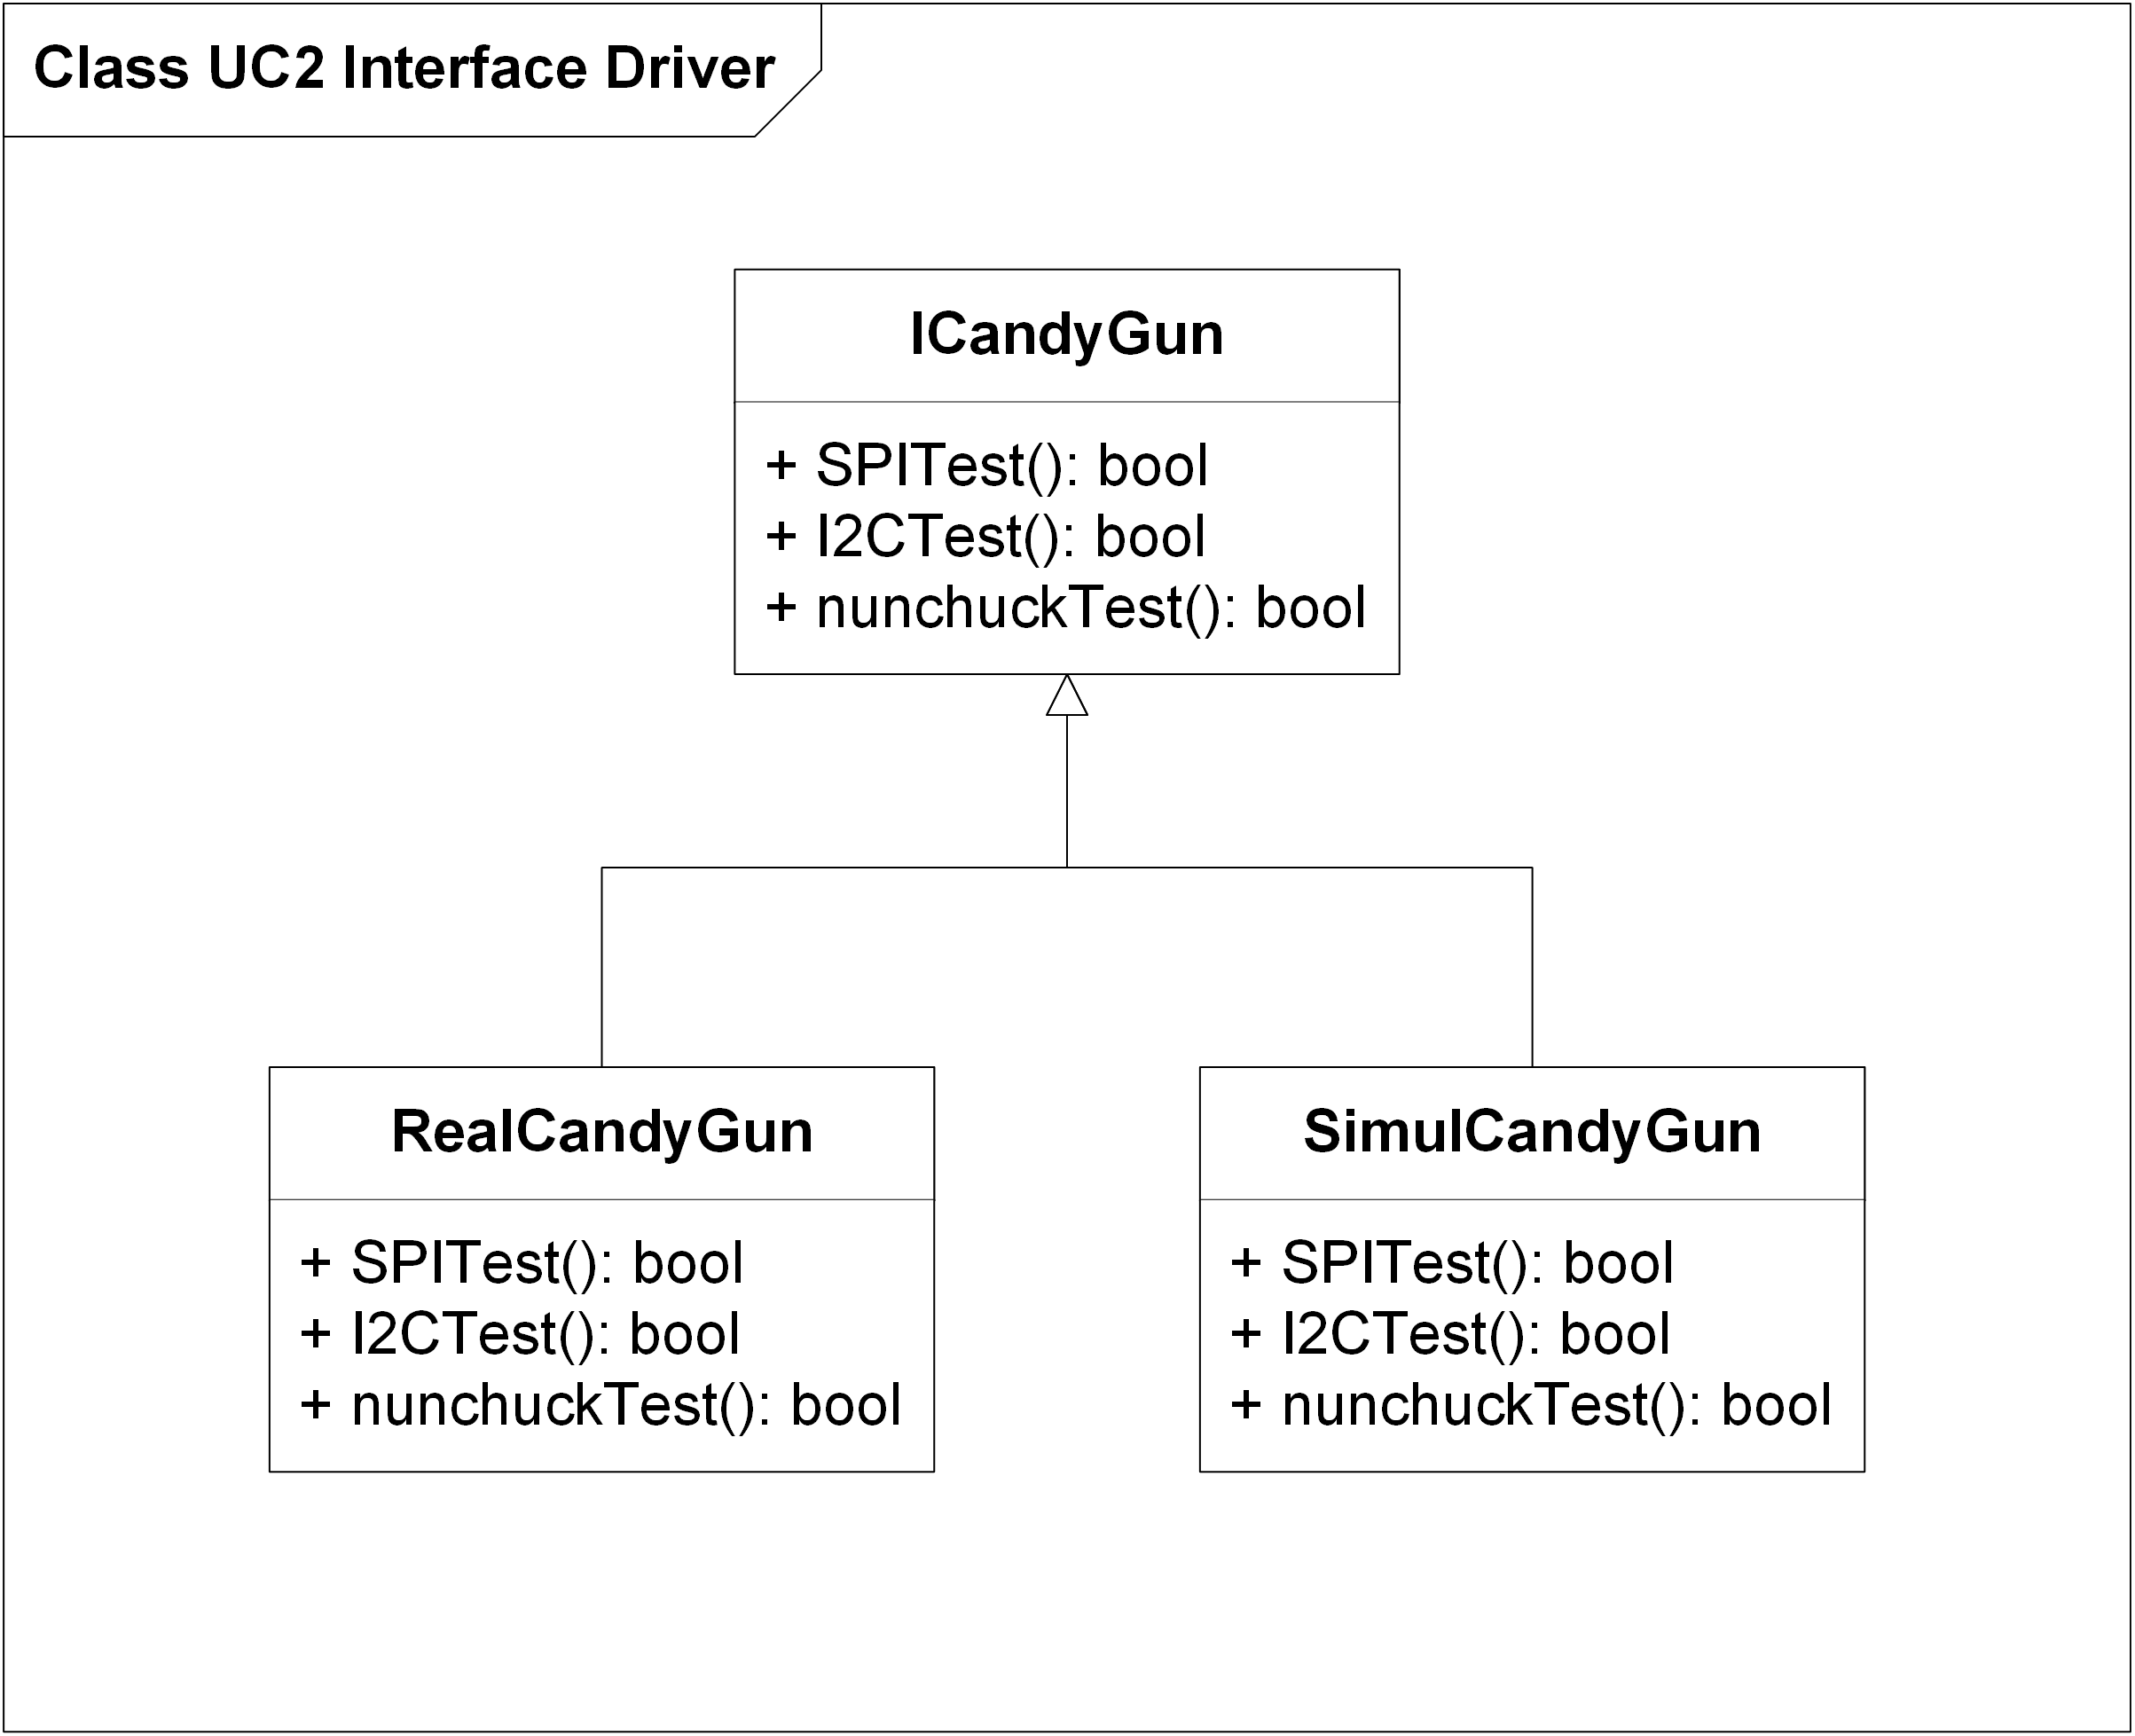
\includegraphics[width=\textwidth]{DesignOgImplementering/images/IdriverKlasseDiagram}
	\caption{Klassediagram for Interface driveren på Devkit8000}
	\label{fig:IDriverKlasseDiagram}
\end{figure}

I det følgende ses tabeller for funktionsbeskrivelse. Funktioner for ICandyGun-klassen er ikke beskrevet, da klassen er abstrakt og alle funktioner dermed er pure virtual. Til gengæld er både funktionerne for SimulCandygun og RealCandyGun beskrevet i hver sin tabel. Bemærk at funktionerne hedder det samme for begge klasser, da de begge er afledede funktioner i et arvehierarki.  
I tabel \ref{idriverFunktioner} ses funktionsbeskrivelser for SimulCandyGun. 

\begin{table}[H]
	\centering
	\caption{My caption}
	\label{idriverFunktioner}
	\begin{tabular}{|l|l|}
		\hline
		\textbf{Metode}      & \textbf{Beskrivelse}                                                                                                     \\ \hline
		SPITest(): bool      & Simulerer resultatet af SPI-testen i systemet. \\ Der anvendes rand() til at returnerer et tilfældigt tal mellem 0 og 1.    \\ \hline
		I2CTest(): bool      & Simulerer resultatet af I2C-testen i systemet. \\ Der anvendes rand() til at returnerer et tilfældigt tal mellem 0 og 1.    \\ \hline
		nunchuckTest(): bool & Simulerer resultatet af nuchucktesten i systemet. \\ Der anvendes rand() til at returnerer et tilfældigt tal mellem 0 og 1. \\ \hline
	\end{tabular}
\end{table}


\subsection{Klassediagrammer}

\subsubsection{PSoC0}
På figur \ref{figure:PSoC0KlasseDiagram} ses klassediagrammet indeholdende klasserne som bruges af softwaren allokeret på CPU'en PSoC0.

\begin{figure}[H]
	\centering
	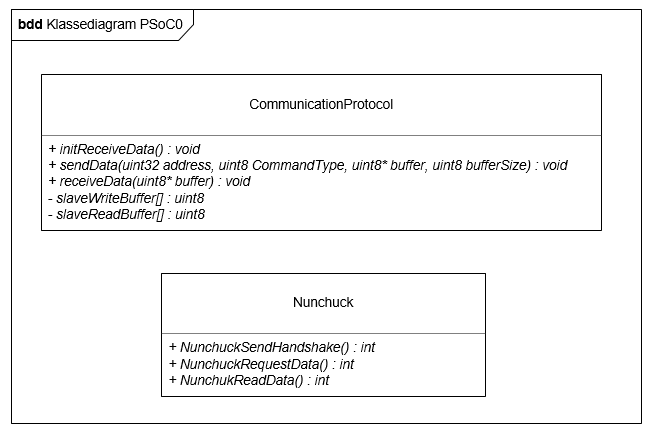
\includegraphics[width=\textwidth]{DesignOgImplementering/images/PSoC0KlasseDiagram}
	\caption{Klassediagram for CPU'en PSoC0}
	\label{figure:PSoC0KlasseDiagram}
\end{figure}

På figur \ref{figure:PSoC0KlasseDiagram} kan det ses at softwaren på PSoC0 CPU'en gør brug af klasserne \textit{CommunicationProtocol} samt \textit{Nunchuck}.

Klassebeskrivelser kan findes i \textbf{!INDSÆT BILAG TIL DOXYGEN!}

\subsection{Afkodning af Wii-Nunchuck Data Bytes}
Aflæste bytes fra Wii-Nunchuck - indeholdende tilstanden af knapperne og det analoge stick - er kodet når de oprindeligt modtages via I2C bussen. Disse bytes skal altså afkodes før deres værdier er brugbare. Afkodningen af hver byte sker ved brug af følgende formel:

\textit{AfkodetByte = (AflæstByte XOR 0x17) + 0x17}

Fra formlen kan det ses at den aflæste byte skal \textit{XOR}'s (Exclusive Or) med værdien 0x17, hvorefter dette resultat skal adderes med værdien 0x17.

\subsection{Kalibrering af Wii-Nunchuck Analog Stick}
De afkodede bytes for Wii-Nunchuck's analoge stick har definerede standardværdier for dets forskellige fysiske positioner. Disse værdier findes i tabel \ref{tabel:WiiNunchuckStickPositioner}

\begin{table}[H]
	\centering
	\begin{tabular}{|l|l|}
		\hline
		X-akse helt til venstre & 0x1E \\ \hline
		X-akse helt til højre   & 0xE1 \\ \hline
		X-akse centreret        & 0x7E \\ \hline
		Y-akse centreret        & 0x7B \\ \hline
		Y-akse helt frem        & 0x1D \\ \hline
		Y-akse helt tilbage     & 0xDF \\ \hline
	\end{tabular}
	\caption{Standardværdier for fysiske positioner af Wii-Nunchuck's analoge stick}
	\label{tabel:WiiNunchuckStickPositioner}
\end{table}

I praksis skal de afkodede værdier for det analoge stick kalibreres, da slør pga. brug gør at de ideale værdier ikke rammes. 

I projektet er de afkodede værdier for det analoge stick kalibreret med værdien -15 (0x0F i hexadecimal), altså ser den endelige formel for afkodning samt kalibrering således ud:

\textit{AfkodetByte = (AflæstByte XOR 0x17) + 0x17 - 0x0F}

\section{Hardwaredesign}
På baggrund af BDD'et er der fundet følgende hardwareblokke, der skal udarbejdes: 
\begin{itemize}
	\item Motorstyring
	\item Tre motorer
	\item Affyringsmekanisme 
\end{itemize}

\subsubsection{Motor}
Der er truffet et valg om at bruge en DC-motor i alle tre tilfælde. De to motorer skal bruges til at styre kanonen i to retninger, og den sidste skal bruges i affyringsmekanismen. 

\subsection{Motorstyring}
Til at styre de tre motorer er der bygget en H-bro, der skal bruges i tre eksemplarer. To af disse motorer skal kunne styre kanonen, så den ene gør at den kan køre op og ned, og den anden gør, at den kan køre fra side til side. Den tredje skal bruges til at styre affyringsmekanismen. 

\subsubsection{H-bro}
Der blev først designet en H-bro, som bestod af to N-MOSFET's af typen IRLZ44 og to P-MOSFET's af typen ZVP3306. Denne kan ses i bilaget. Det viste sig dog, at den P-MOSFET, der var brugt, var for svag til at kunne trække den strøm, som motoren skulle bruge, hvilket betød, at den blev brændt af. Derfor blev denne H-bro modificeret, så de to P-MOSFET's blev udskiftet med to MOSFET's af typen IRF9Z34N, der kan trække en større strøm. 

\begin{figure}[H]
	\centering
	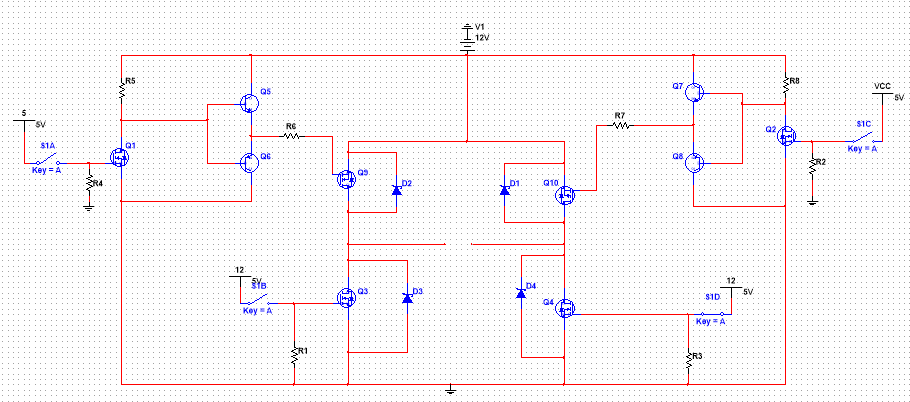
\includegraphics[width=\textwidth]{DesignOgImplementering/images/motorkreds}
	\caption{Kredsløb for H-bro}
	\end{figure}

\begin{table}[]
	\centering
	\caption{Komponentbetegnelser på H-bro}
	\label{my-label}
	\begin{tabular}{|l|l|l}
		\cline{1-2}
		Betegnelse 	& Komponent 	          	 &  \\ \cline{1-2}
		VCC        	& 5V                         &  \\ \cline{1-2}
		Q1   		& IRLZ44(mosfet N-Channel)   &  \\ \cline{1-2}
		Q2   		& IRLZ44(mosfet N-Channel)   &  \\ \cline{1-2}
		Q3   		& IRLZ44(mosfet N-Channel)   &  \\ \cline{1-2}
		Q4   		& IRLZ44(mosfet N-Channel)   &  \\ \cline{1-2}
		Q5   		& BC547                      &  \\ \cline{1-2}
		Q6   		& BC557                      &  \\ \cline{1-2}
		Q7   		& BC547                      &  \\ \cline{1-2}
		Q8   		& BC557                      &  \\ \cline{1-2}
		Q9   		& IRF9Z34N(mosfet P-Channel) &  \\ \cline{1-2}
		Q10  		& IRF9Z34N(mosfet P-Channel) &  \\ \cline{1-2}
		R1   		& 10k$\Omega$                &  \\ \cline{1-2}
		R2   		& 10k$\Omega$                &  \\ \cline{1-2}
		R3   		& 10k$\Omega$                &  \\ \cline{1-2}
		R4   		& 10k$\Omega$                &  \\ \cline{1-2}
		R5   		& 10k$\Omega$                &  \\ \cline{1-2}
		R6   		& 100$\Omega$                &  \\ \cline{1-2}
		R7   		& 100$\Omega$                &  \\ \cline{1-2}
		R8   		& 10k$\Omega$                &  \\ \cline{1-2}
		D1   		& IN5819                     &  \\ \cline{1-2}
		D2   		& IN5819                     &  \\ \cline{1-2}
		D3   		& IN5819                     &  \\ \cline{1-2}
		D4   		& IN5819                     &  \\ \cline{1-2}
	\end{tabular}
\end{table}

\subsubsection{MOSFET'er}
Til at styre motoren er der bygget en H-bro, som består af fire mosfet, hvor to af dem er af typen IRF9Z34N (mosfet P-channel, som er Q9 og Q10 på kredsløbstegningen) og de to andre mosfet er af typen IRLZ44 (mosfet N-Channel, som er Q3 og Q4 kredsløbstegningen). Det er valgt at bruge mosfet for at kunne styre H-broen, da det ved denne er muligt at lukke og åbne for spændingen, og de bliver styret af spænding, i forhold til transistorer, som bliver styret af strøm. 

\begin{itemize}
\item MOSFET N-kanal\\
	Der er i denne H-bro brugt en N-kanals-MOSFET af typen IRLZ44. Denne MOSFET skal bruges til at trække strømmen fra den tilsvarende P-MOSFET til stel, så motoren kan begynde at køre. Det sker, når der kommer 5V ind på gate-benet. 
	\\MOSFET'en fungerer på den måde, at når der kommer positiv spænding ind på gate-benet åbner den, så der kommer forbindelse til stel og når der kommmer 0V ind på dette lukker den igen. 
	
	\begin{figure}[H]
		\centering
		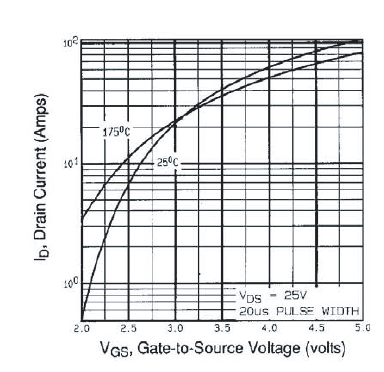
\includegraphics[width=\textwidth]{DesignOgImplementering/images/grafn}
		\caption{Gate-to-Source Voltage REFERENCE TIL DATABLAD HER!!!!}
	\end{figure}
	
	På figur (reference her!) ses det, at når der er en gate-to-source-spænding på 5V, vil der MOSFET'en kunne klare, at der løber en strøm på op til 100A/30A (TJEK DETTE!!). Det vil altså ikke komme til at påvirke motoren, da denne kun kan trække en strøm på cirka 0,35A. 
	
\item MOSFET P-kanal \\
	Der er valgt at bruge en P-MOSFET af typen IRF9Z34N. Denne MOSFET skal bruges til at trække de 12V ned til motoren, så denne kan køre. Samtidig sørger den for, at de 12V ikke løber ned til motoren så længe, der ikke er negativ spænding på gate-benet. 
	Denne type MOSFET kan trække en strøm på 6,7A ifølge databladet. Det vil altså ikke komme til at påvirke motoren, da den kun kan trække en strøm på cirka 0,35A. 
	
	For at der kan løbe spænding igennem IRF9Z34N, skal den have en negativ spænding for at åbne og en spænding på over 0V for at lukke. 
		
	\begin{figure}[H]
		\centering
		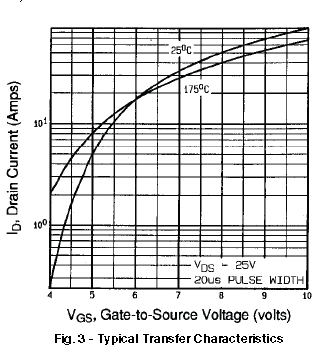
\includegraphics[width=\textwidth]{DesignOgImplementering/images/grafp}
		\caption{Gate-to-Source Voltage REFERENCE TIL DATABLAD HER!!!!}
	\end{figure}
	
	På figuren (REFERENCE HER!) ses det, at når der er en gate-to-source-spænding på 5V, vil derr kunne løbe en strøm på omkring 5A igennem MOSFET'en, hvilket er mere end nok til at få motoren til at køre. 
	
\end{itemize}

\subsubsection{Dioder}
Over fire af mosfetene (Q9, Q10, Q3 og Q4) er der sat en diode af typen IN5819. Den skal fungere som beskyttelse af de fire mosfet (Q9, Q10, Q3 og Q4). Det, de gør, er, at de sikrer, at den spænding, som er tilbage i motoren, når man lukker for mosfetene, ikke løber tilbage ind i mosfetene og brænder dem af.

\subsubsection{Modstande}
\begin{itemize}
	\item Pull down modstande:\\
	Der er blevet brugt fire pull-down-modstande (R1, R2, R3 og R4). Disse sørger for, at signalet vil blive holdt lavt, når der ikke er trykket, så dette ben ikke står og flyver, så det kan komme til at åbne en mosfet ved en fejl og derved kommer til at brænde en mosfet eller motoren af. Der er valgt en modstand på 10 kOhm, hvilket betyder, at den er lille nok til at trække de små spændinger ned, når der ikke er trykket, og den stor nok til at spændingen ikke løber derned, når der er trykket. 
	\item Andre modstande
	\begin{itemize}
		\item R6 og R7\\
			Grunden til, at R6 og R7 er der, er for at sikre, at transistorernes Absolute Maximum Ratings omkring strømmen, som ikke må overstige 100mA ifølge databladet. (tjek lige om det er rigtig)
		\item R5 og R8\\
			Grunden til at R5 og R8 er sat ind i kredsløbet er, at der ifølge databladet kun kan løbe en strøm på omkring 30A igennem den N-MOSFET, der er brugt, Vgs er 10V. Da Vgs kun er sat til 5V, vil MOSFET'en altså ikke kunne klare en alt for stor strøm. Derfor er R5 og R8 sat ind for at forhindre, at MOSFET'en ikke brænder af. 
	\end{itemize}

\end{itemize}

\subsubsection{Transistorer}
\begin{itemize}
	\item Q5 og Q7
	Disse transistorer sidder i kredsløbet, fordi det tager tid for N-MOSFET'en at åbne helt. Det hjælper den ene af disse transistorer til med. 
	
	\item Q6 og Q8
	Disse to transistorer sidder der for at hjælpe med at lukke N-MOSFET'en igen. Inden Q5 og Q7 blev sat ind tog det ingen tid for at lukke N-MOSFET'en, men da de to blev sat ind påvirkede det lige pludselig lukketiden. Derfor sidder de der, for at IRLZ44 kan lukke hurtigt. 
\end{itemize}


